\documentclass{article}

\usepackage[english]{babel}
\usepackage[utf8]{inputenc}
\usepackage{amsmath}
\usepackage{amsthm}
\usepackage{amssymb}
\usepackage{amsfonts}
\usepackage{bbm}
\usepackage{graphicx}
\usepackage{wrapfig}

% set up margin
\usepackage
[
  a4paper,
  left=3cm,
  right=3cm,
  top=3cm,
  bottom=3cm,
]
{geometry}

% set up header
\usepackage{fancyhdr}
\pagestyle{fancy}
\fancyhf{}
\lhead{6.438 Algorithms for Inference}
\chead{Problem Set 1}
\rhead{Hongzi Mao}
\cfoot{\thepage}

% footer line
\renewcommand{\footrulewidth}{0.4pt}

% sans serif italic
\newcommand{\s}[1]{\textsf{\textit{#1}}}

% set symbol
\usepackage[mathscr]{euscript}

% empty set
\let\emptyset\varnothing

% qed
\newcommand{\qeds}{\hfill\qedsymbol}

% independence symbol
\makeatletter
\newcommand*{\indep}{%
  \mathbin{%
    \mathpalette{\@indep}{}%
  }%
}
\newcommand*{\nindep}{%
  \mathbin{%                   % The final symbol is a binary math operator
    \mathpalette{\@indep}{\not}% \mathpalette helps for the adaptation
                               % of the symbol to the different math styles.
  }%
}
\newcommand*{\@indep}[2]{%
  \sbox0{$#1\perp\m@th$}%        box 0 contains \perp symbol
  \sbox2{$#1=$}%                 box 2 for the height of =
  \sbox4{$#1\vcenter{}$}%        box 4 for the height of the math axis
  \rlap{\copy0}%                 first \perp
  \dimen@=\dimexpr\ht2-\ht4-.2pt\relax
  \kern\dimen@
  {#2}
  \kern\dimen@
  \copy0 %                       second \perp
} 
\makeatother

%%%%%%%%%%%%%%%%%%%%%%%%%%%%%%%%%%%%%%%%%%%%%%%%%%%%%%%%%%%%%%%%%%%%%%%%
%%%%%%%%%%%%%%%%%%%%%%%%% Begin document here %%%%%%%%%%%%%%%%%%%%%%%%%%
%%%%%%%%%%%%%%%%%%%%%%%%%%%%%%%%%%%%%%%%%%%%%%%%%%%%%%%%%%%%%%%%%%%%%%%%
\begin{document}
 
\section*{Problem 1}
(a) Let $\s{x} = \s{z}\s{w}_1$ and $\s{y} = \s{z}\s{w}_2$.
%
From the directed graphical model in Figure~\ref{f:1a},
we have $\s{x} \nindep \s{y}$ while $\s{x} \indep \s{y} | \s{z}$.

\begin{figure}[h]
  \centering
  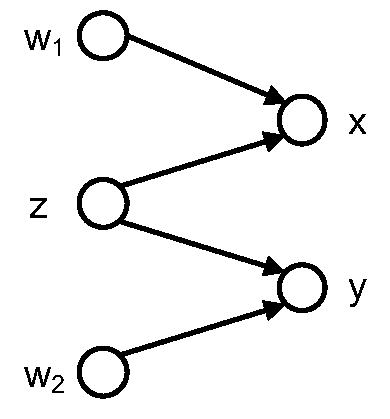
\includegraphics[width=0.2\columnwidth]{1a.pdf}
  \caption{Directed graphical model for 1(a).}
  \label{f:1a}
\end{figure}

We can also see the conditionality with an example. Let $z\in\{-1, 1\}$ and
$w_1, w_2 \in\{0, 1\}$. Now,  knowing the sign of $x$ immediately
unveils the sign of $y$, which means $\s{x} \nindep \s{y}$. However,
condition on the sign of $z$, the value of $x$ does not influence (i.e.,
unveil information) of $y$. Thus, $\s{x} \indep \s{y} | \s{z}$.
\\

\noindent
(b) ``$\Longrightarrow$'':
\\

Since
\begin{align*}
p_{\s{x}, \s{y}, \s{z}}(x, y, z) &= p_{\s{x}, \s{y} | \s{z}}(x, y | z) p_{\s{z}}(z)\\
&= p_{\s{x}| \s{z}}(x | z) p_{\s{y}| \s{z}}(y | z) p_{\s{z}}(z),
\end{align*}
%
we can assign $h(x, z) = p_{\s{x}| \s{z}}(x | z)$ and 
$g(y, z) = p_{\s{y}| \s{z}}(x | z) p_{\s{z}}(z)$.
\\

``$\Longleftarrow$'':
\\

By marginalizing $\s{x}$ and $\s{y}$,
\begin{align*}
	p_{\s{x}|\s{z}}(x|z) &= \sum_y p_{\s{x}, \s{y}|\s{z}}(x, y|z)\\
	&= \sum_y \frac{p_{\s{x}, \s{y}, \s{z}}(x, y, z)}{p_{\s{z}}(z)}\\
	& = \frac{h(x, z)}{p_{\s{z}}(z)} \sum_y  g(y, z),
\end{align*}
\begin{align*}
	p_{\s{y}|\s{z}}(y|z) &= \sum_x p_{\s{x}, \s{y}|\s{z}}(x, y|z)\\
	&= \sum_x \frac{p_{\s{x}, \s{y}, \s{z}}(x, y, z)}{p_{\s{z}}(z)}\\
	& = \frac{g(y, z)}{p_{\s{z}}(z)} \sum_x  h(x, z).
\end{align*}

Since \, $\sum_x p_{\s{x}|\s{z}}(x|z) = 1$,
\begin{equation*}
	\frac{\sum_x h(x, z) \sum_y g(y, z)}{p_{\s{z}}(z)} = 1.
\end{equation*}

Thus,
\begin{align*}
	p_{\s{x}|\s{z}}(x|z)p_{\s{y}|\s{z}}(y|z) &= \frac{h(x, z)}{p_{\s{z}}(z)} \sum_y  g(y, z)\frac{g(y, z)}{p_{\s{z}}(z)} \sum_x  h(x, z) \\
	&= \frac{\sum_x h(x, z) \sum_y g(y, z)}{p_{\s{z}}(z)} \frac{h(x, z) g(y, z)}{p_{\s{z}}(z)}\\
	&= \frac{h(x, z) g(y, z)}{p_{\s{z}}(z)} \\
	&= \frac{p_{\s{x}, \s{y}, \s{z}}(x, y, z)}{p_{\s{z}}(z)} \\
	&= p_{\s{x},\s{y}|\s{z}}(x, y|z).
\end{align*} \qeds
\pagebreak

%%%%%%%%%%%%%%%%%%%%%%%%%%%%%%%%%%%%%%%%%%%%%%%%%%%%%%%%%%%%%%%%%%%%%%%%

\section*{Problem 2}
(a)
%
Since $\mathscr{S}$ is a finite set, for convenience and without loss of generality,
we can write $\mathscr{S} = \{1, 2, ..., N\}$, where $N = |\mathscr{S}|$.

In preparation, we compute
$\gamma(1) = \mu(1)$, $\gamma(2) = \mu(1) + \mu(2)$, $\dots$,
$\gamma(N) = \mu(1) + \mu(2) + \dots + \mu(N) = 1$.
Let $\gamma(0) = 0$.
This preparation step takes $O(|\mathscr{S}|)$.

Notice
\begin{align*}
\mathbb{P}\Big(0 \leq UN \leq \gamma(1)\Big) &= \mu(1), \\
\mathbb{P}\Big(\gamma(1) < UN \leq \gamma(2)\Big) &= \mu(2), \\
	& \cdots \\
\mathbb{P}\Big(\gamma(i - 1) < UN \leq \gamma(i)\Big) &= \mu(i), \\	
	& \cdots \\
\mathbb{P}\Big(\gamma(N - 1) < UN \leq 1\Big) &= \mu(N). \\
\end{align*}

Thus, we sample $U \sim \text{unif}([0, 1])$, check which interval $UN$ falls in (i.e., sandwiched by which $\gamma$ interval). The $\gamma(i)$ interval $UN$ falls in corresponds to the index $i$ of element in $\mathscr{S}$ to output. This takes $O(|\mathscr{S}|)$ to check, as there are $N$ such intervals.
\\

%
\noindent
(b) Notice
\begin{align*}
p(x_1, x_2, \cdots, x_n) &= p(x_1 | x_2, \cdots, x_n) \; p(x_2 | x_3, \cdots, x_n)\; \cdots
p(x_{n-1}|x_n)\;p(x_n)\\
&= \frac{p(x_1, x_2, \cdots, x_n)}{p(x_2, x_3, \cdots, x_n)}
\frac{p(x_2, x_3, \cdots, x_n)}{p(x_3, x_4, \cdots, x_n)}
\cdots\frac{p(x_{n-1})}{p(x_n)}p(x_n).
\end{align*}

Now, from the black-box A we have access to arbitrary marginals,
which means we can compute each of the nominators and denominators above.
Thus, we can compute each term of the above telescoping factorization.
This involves $2n -1 = O(n)$ calls of black-box A.

Notice that we sample the term from right to left, so we can invoke (a) \emph{independently} n times. Therefore the computation
time is now $O(n|\mathscr{X}|)$.
\\

%
\noindent
(c) We consider two sets of cliques in $\mathscr{G}$
\begin{align*}
\mathcal{A} &= \Big\{\mathscr{C}: \mathscr{C} \in cl(\mathscr{G}), \mathscr{C}\cap\{1\} = \emptyset \Big\},\\
\mathscr{B} &= \Big\{\mathscr{C}: \mathscr{C} \in cl(\mathscr{G}), \mathscr{C}\cap\{1\} \neq \emptyset \Big\}.
\end{align*}
\\
%
Since
\begin{align*}
p_{\s{x}_1, \s{x}_2, \cdots, \s{x}_n}(x_1, x_2, \cdots, x_n) = p_{\s{x}_2, \s{x}_3, \cdots, \s{x}_n | \s{x}_1}(x_2, x_3, \cdots, x_n | x_1) \,p_{\s{x}_1}(x_1),
\end{align*}
we know the conditional distribution is proportional to the original distribution (as $p_{\s{x}_1}(x_1)$ can be absorbed in partition function $Z$). Thus the multiplications of potentials over cliques should carry over to the new graph.

Now, in the new undirected graph $\mathscr{G}'$ with all edges involving node 1 removed, the set of cliques still contain $\mathscr{A}$, since no edges are removed from $\mathscr{A}$. Thus for $\mathscr{C}\in\mathscr{A}$,
\begin{align*}
\psi'_{\mathscr{C}\in\mathscr{A}}(x_{\mathscr{C}}) =
\psi_{\mathscr{C}\in\mathscr{A}}(x_{\mathscr{C}}),	
\end{align*}
where $\psi$ is the potential function in the original graph $\mathscr{G}$, and $\psi'$ is on the new graph $\mathscr{G}'$.

For the rest of the cliques in $\mathscr{G}'$, i.e., $\mathscr{B}' = \Big\{\mathscr{C}: \mathscr{C} \in cl(\mathscr{G}'), \mathscr{C} \not\in \mathscr{A}\Big\}$, each clique maps to the clique in $\mathscr{B}$ with edges to node 1 removed. Thus, the relation of the potential functions is
\begin{align*}
\psi'_{\mathscr{C}\in\mathscr{B}'}(x_{\mathscr{C}}) = \psi_{\mathscr{C}\in\mathscr{B}}(x_{\mathscr{C} \backslash \{1\}}, x_1).	
\end{align*}
Intuitively, the new potential corresponds to the old one with $x_1$ actualized in the node.
\\

%
\noindent
(d) Similar to (b) we expand
\begin{align*}
p(x_1, x_2, \cdots, x_n) &= p(x_1 | x_2, \cdots, x_n) \;
p(x_2 | x_3, \cdots, x_n)\; \cdots
p(x_{n-1}|x_n)\;p(x_n).
\end{align*}
Now, from right to left, we first invoke black-box B on node $n$ to get
the marginal distribution of $p(x_n)$. Next, we use (c) to update the graph
by removing edges connect to $n$ and update the corresponding potential ($x_n$ is fixed, as we are now sampling $x_{n-1}$).
Then on the new graph, we invoke black-box B on node $n-1$ to get 
marginal distribution of $p(x_{n-1}|x_n)$. This defines an iterative algorithm.

More concretely, at iteration step $i$, we first remove edges connect to
node $n - i + 1$; use (c) to update the potential; and then invoke black-box
B on node $n-i$ to get the marginal distribution $p(x_{n-i+1}|x_{n-i},
\cdots, x_n)$.

The whole algorithm makes $n=O(n)$ calls to black-box B and takes
$O(n|\mathscr{X}|)$ to sample ($\s{x}_1, \s{x}_2, \cdots, \s{x}_n$).

\pagebreak
%%%%%%%%%%%%%%%%%%%%%%%%%%%%%%%%%%%%%%%%%%%%%%%%%%%%%%%%%%%%%%%%%%%%%%%%

\section*{Problem 3}
(a)(i) From the given values of $p(x_1, x_2, x_3, x_4)$, we see
\begin{align*}
p(1,0,0,0) &= p(0,0,0,1) = 1/8, \\
p(1,1,0,0) &= p(0,0,1,1) = 1/8, \\
p(1,1,1,0) &= p(0,1,1,1) = 1/8, \\
p(0,0,0,0) &= p(0,0,0,0) = 1/8, \\
p(1,1,1,1) &= p(1,1,1,1) = 1/8,
\end{align*}
and all other combinations are all with 0 probability.
Thus, $p(x_1, x_2, x_3, x_4) = (x_4, x_3, x_2, x_1)$. \qeds
\\

%
\noindent
(ii) Notice that
\begin{align*}
(x_2, x_4) = (0, 0) &\Longrightarrow	 x_3 = 0,\\
(x_2, x_4) = (1, 0) &\Longrightarrow	 x_1 = 1,\\
(x_2, x_4) = (0, 1) &\Longrightarrow	 x_1 = 0,\\
(x_2, x_4) = (1, 1) &\Longrightarrow	 x_3 = 1,
\end{align*}
while the other value in $x_1$ or $x_3$ is undetermined. Thus, this proves 
$x_1 \indep x_3 | x_2, x_4$. \qeds
\\

%
\noindent
(b) Assume Hammersley-Clifford factorization exists, then
\begin{align*}
p(0, 0, 0, 0) &= \phi_{12}(0,0)\;\phi_{23}(0,0)\;\phi_{34}(0,0)\;\phi_{41}(0,0)=1/8,\\
p(0, 0, 1, 0) &= \phi_{12}(0,0)\;\phi_{23}(0,1)\;\phi_{34}(1,0)\;\phi_{41}(0,0)=0,\\
p(0, 0, 1, 1) &= \phi_{12}(0,0)\;\phi_{23}(0,1)\;\phi_{34}(1,1)\;\phi_{41}(0,0)=1/8,\\
p(1, 1, 1, 0) &= \phi_{12}(1,1)\;\phi_{23}(1,1)\;\phi_{34}(1,0)\;\phi_{41}(0,1)=1/8.
\end{align*}

Here, $p(0, 0, 1, 0) = 0$ means one of the terms in $\phi_{12}(0,0)\;\phi_{23}(0,1)\;\phi_{34}(1,0)\;\phi_{41}(0,0)$ needs to equal $0$.

However,
$\phi_{12}(0,0) \neq 0$ because otherwise $p(0, 0, 0, 0)$ would have been $0$;
$\phi_{23}(0,1) \neq 0$ because otherwise $p(0, 0, 1, 1)$ would have been $0$;
$\phi_{34}(1,0) \neq 0$ because otherwise $p(1, 1, 1, 0)$ would have been $0$;
$\phi_{41}(0,0) \neq 0$ because otherwise $p(0, 0, 1, 1)$ again would have been $0$.
This contradicts with the assumption. \qeds
\pagebreak

%%%%%%%%%%%%%%%%%%%%%%%%%%%%%%%%%%%%%%%%%%%%%%%%%%%%%%%%%%%%%%%%%%%%%%%%

\section*{Problem 4}
(a) The diagram of the undirected graphical model is shown in Figure~\ref{f:4a}.
We write the potential as
\begin{align*}
p_{\s{x}, \s{t}}(x, t) = \psi_{\s{x}, \s{t}}(x, t) = \mathbbm{1}_{x=1}\,p_{\s{t}}(t)\,c_t + \mathbbm{1}_{x=0}\,p_{\s{t}}(t)\,(1 - c_t).
\end{align*}
\begin{figure}[h]
  \centering
  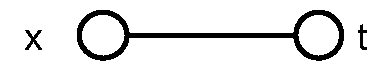
\includegraphics[width=0.2\columnwidth]{4a.pdf}
  \caption{Undirected graphical model for 4(a).}
  \label{f:4a}
\end{figure}
\\

%
\noindent
(b) The diagram of the undirected graphical model is shown in Figure~\ref{f:4b}.
The potential function between $\s{x}$ and $\s{t}$, $\psi_{\s{x}, \s{t}}(x, t)$,
is the same as (a).
We write the potential between $\s{t}$ and each $\s{y}_i$ as
\begin{align*}
\psi_{\s{t}, \s{y}_i}(t, y_i) = p_{\s{t}}(t)\,\exp\left[\sum_{k=1}^K\mathbbm{1}_{t=k}\,\theta_i^k\,y_i\right].
\end{align*}

\begin{figure}[h]
  \centering
  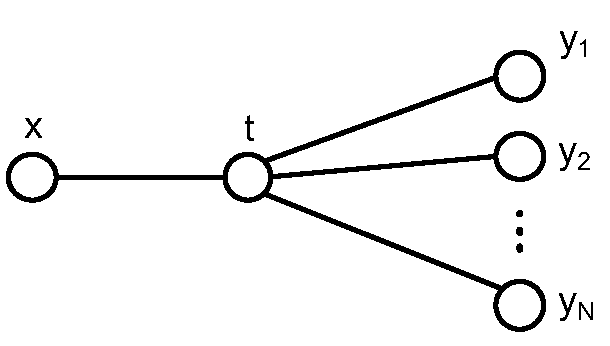
\includegraphics[width=0.3\columnwidth]{4b.pdf}
  \caption{Undirected graphical model for 4(b).}
  \label{f:4b}
\end{figure}
\end{document}